% !TeX root = ../Thesis.tex

%********************************************************************
% Survey (Appendix)
%*******************************************************
% -- TemplateKnob
% If problems with the headers: get headings in appendix etc. right
%\markboth{\spacedlowsmallcaps{Appendix}}{\spacedlowsmallcaps{Appendix}}
\chapter{Survey}\label{ch:survey}
\glsresetall % Resets all acronyms to not used

We implement \gls{HiPS} to perform steganography in chat messages using local \glspl{LLM} on Android smartphones. We are able to influence the encoding of secret messages into cover texts via multiple parameters. In particular, we expose a system prompt in the \gls{UI}. To evaluate cover text quality, we conducted a survey amongst students of TU Darmstadt (see \cref{ch:evaluation}). \cref{fig:survey} shows the chat conversations we used in the survey, both real and cover texts. \cref{tab:systemPrompts} shows the system prompts we used to generate the respective cover texts. Future research can use the insights from our survey to refine these system prompts further.

\begin{figure}
	\captionsetup{width=\linewidth}

	\begin{subfigure}{0.3\linewidth}
		\centering
		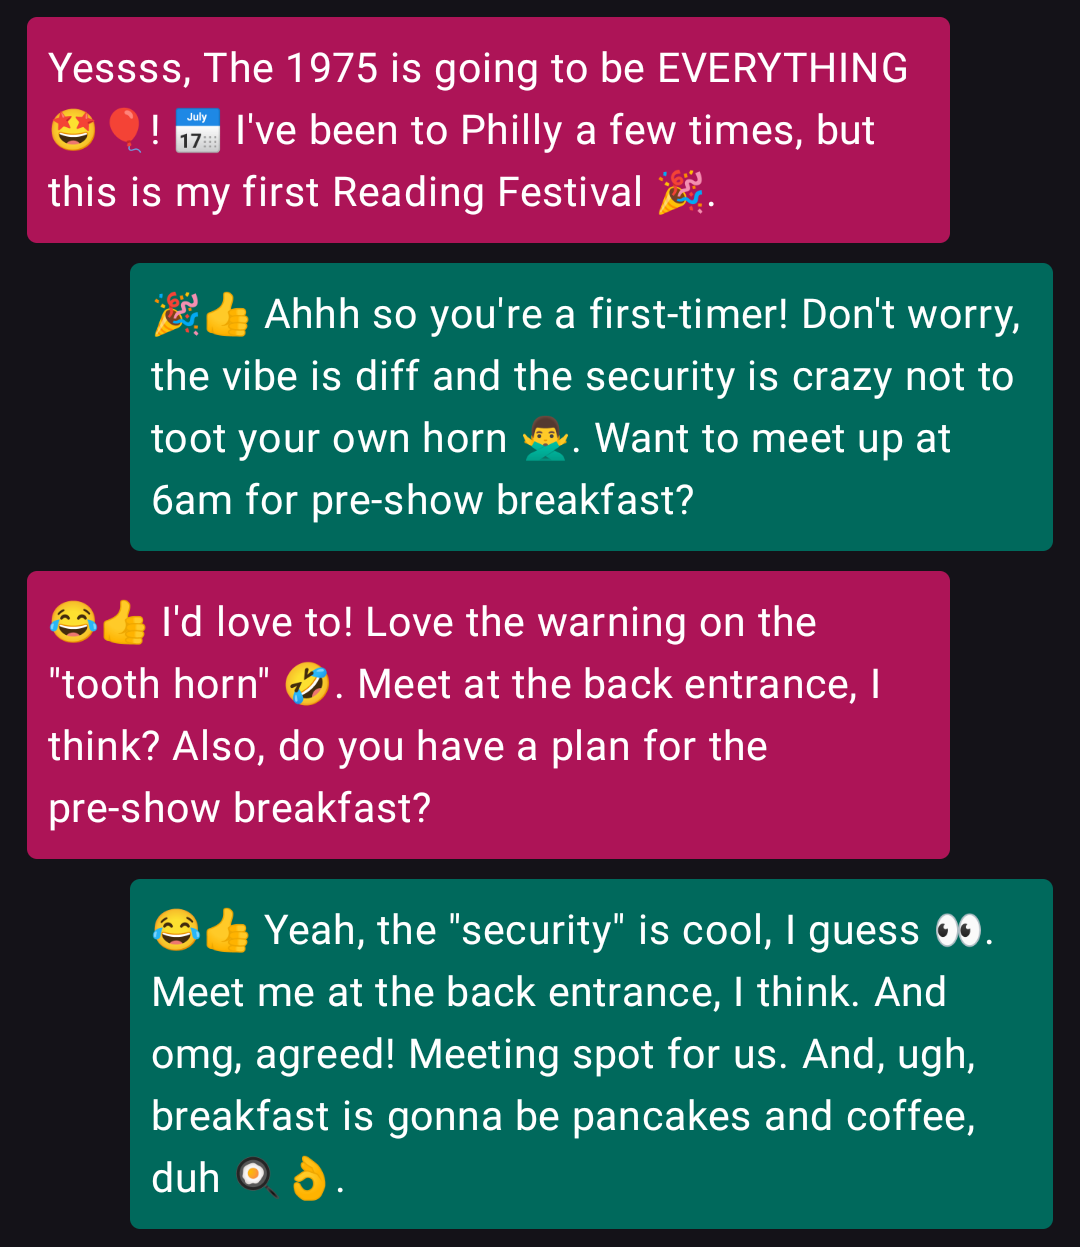
\includegraphics[width=\linewidth]{survey_arithmetic_1.png}
		\caption{Cover texts from Arithmetic coding.}
		\label{fig:surveyArithmetic1}
	\end{subfigure}
	\hfill
	\begin{subfigure}{0.3\linewidth}
		\centering
		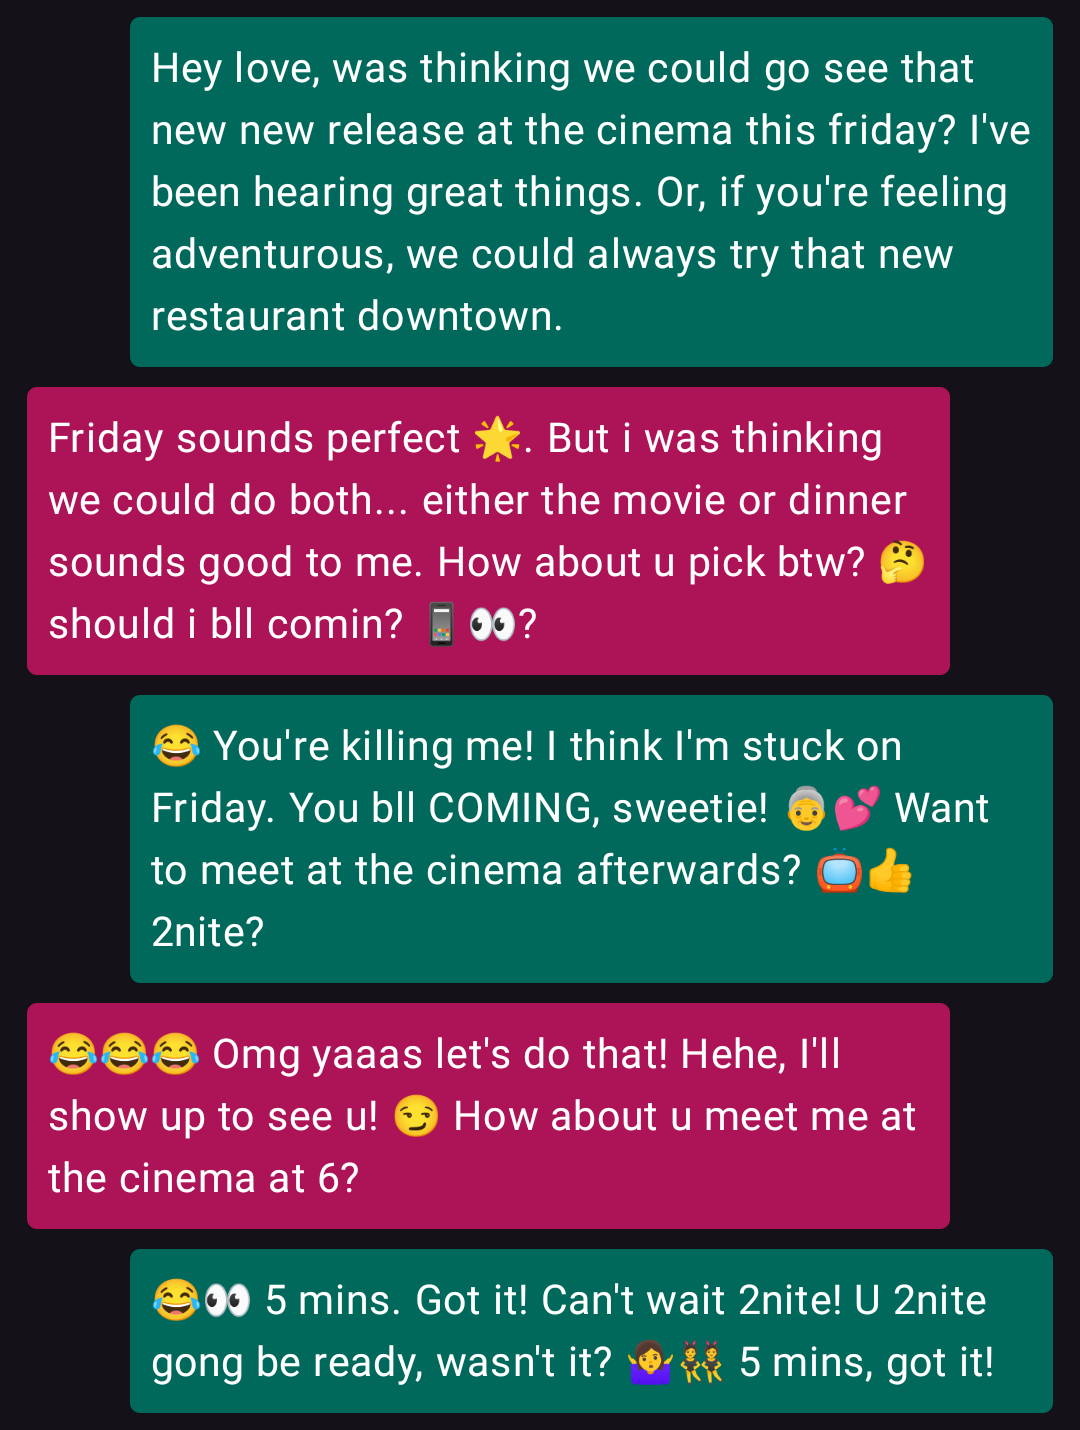
\includegraphics[width=\linewidth]{survey_arithmetic_2.png}
		\caption{Cover texts from Arithmetic coding.}
		\label{fig:surveyArithmetic2}
	\end{subfigure}
	\hfill
	\begin{subfigure}{0.3\linewidth}
		\centering
		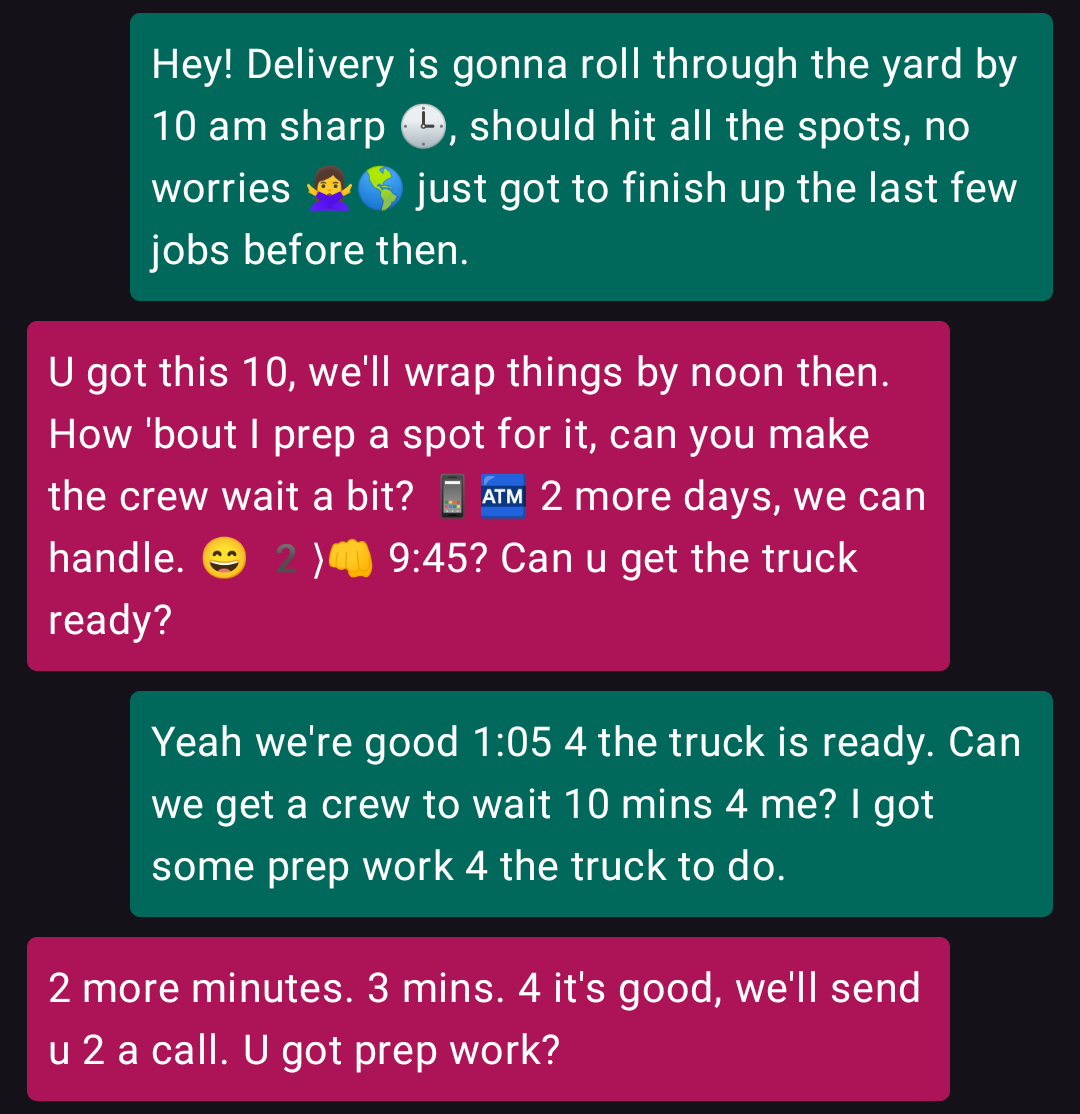
\includegraphics[width=\linewidth]{survey_huffman_1.png}
		\caption{Cover texts from Huffman coding.}
		\label{fig:surveyHuffman1}
	\end{subfigure}

	\begin{subfigure}{0.3\linewidth}
		\centering
		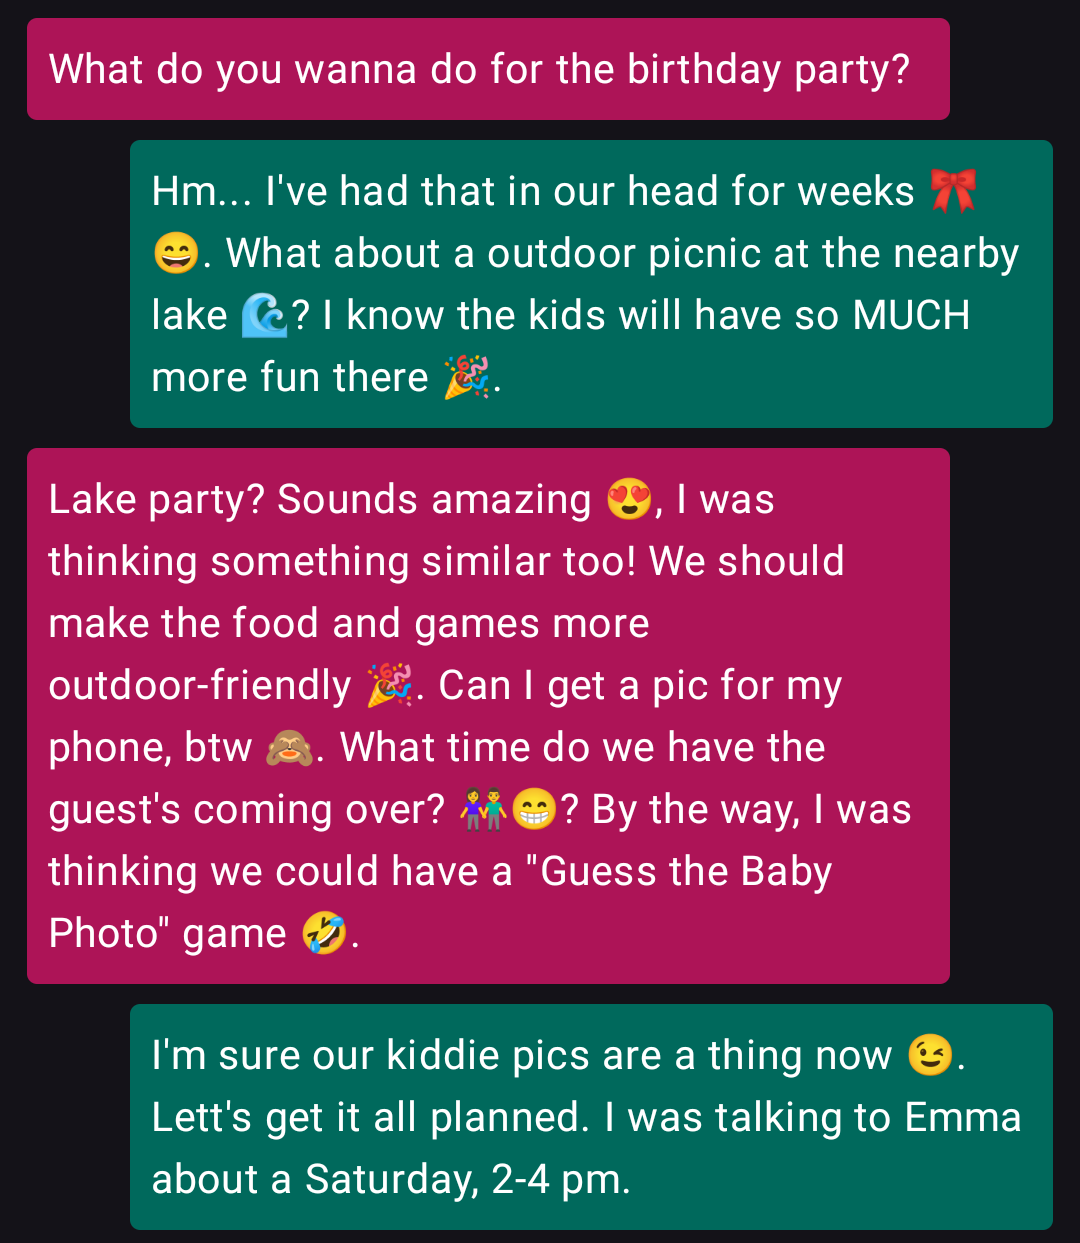
\includegraphics[width=\linewidth]{survey_huffman_2.png}
		\caption{Cover texts from Huffman coding.}
		\label{fig:surveyHuffman2}
	\end{subfigure}
	\hfill
	\begin{subfigure}{0.3\linewidth}
		\centering
		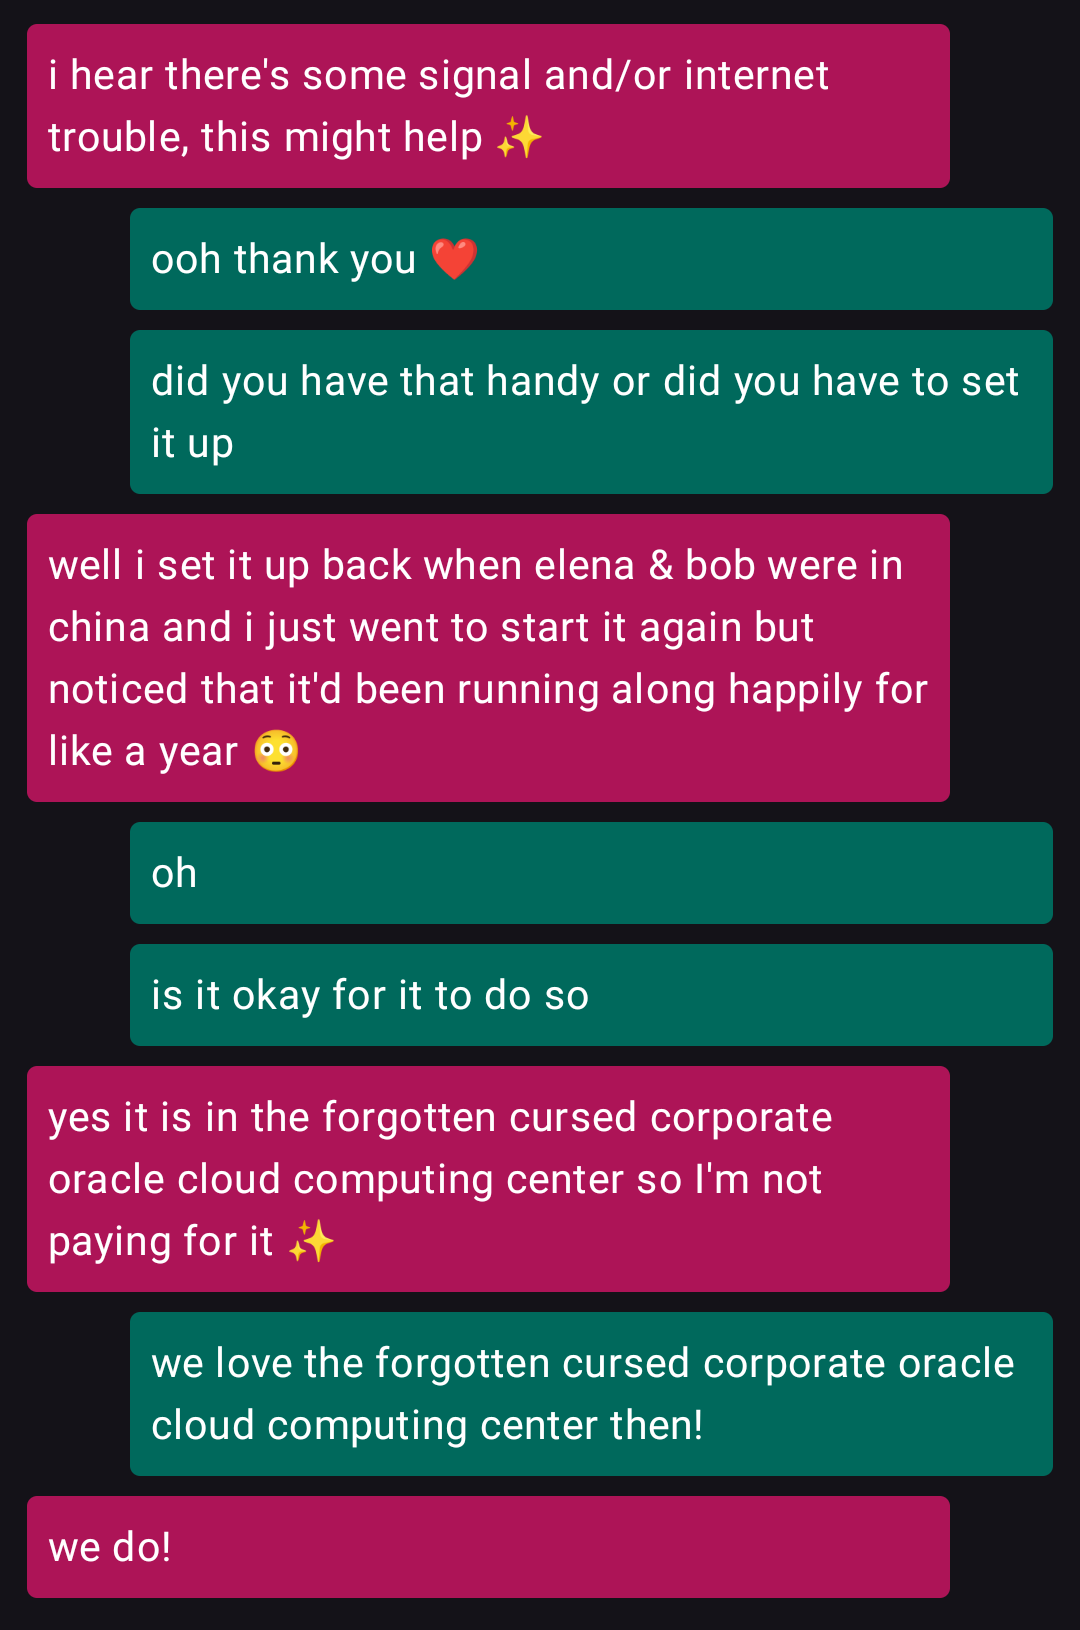
\includegraphics[width=\linewidth]{survey_real_1.png}
		\caption{Real chat conversation.}
		\label{fig:surveyReal1}
	\end{subfigure}
	\hfill
	\begin{subfigure}{0.3\linewidth}
		\centering
		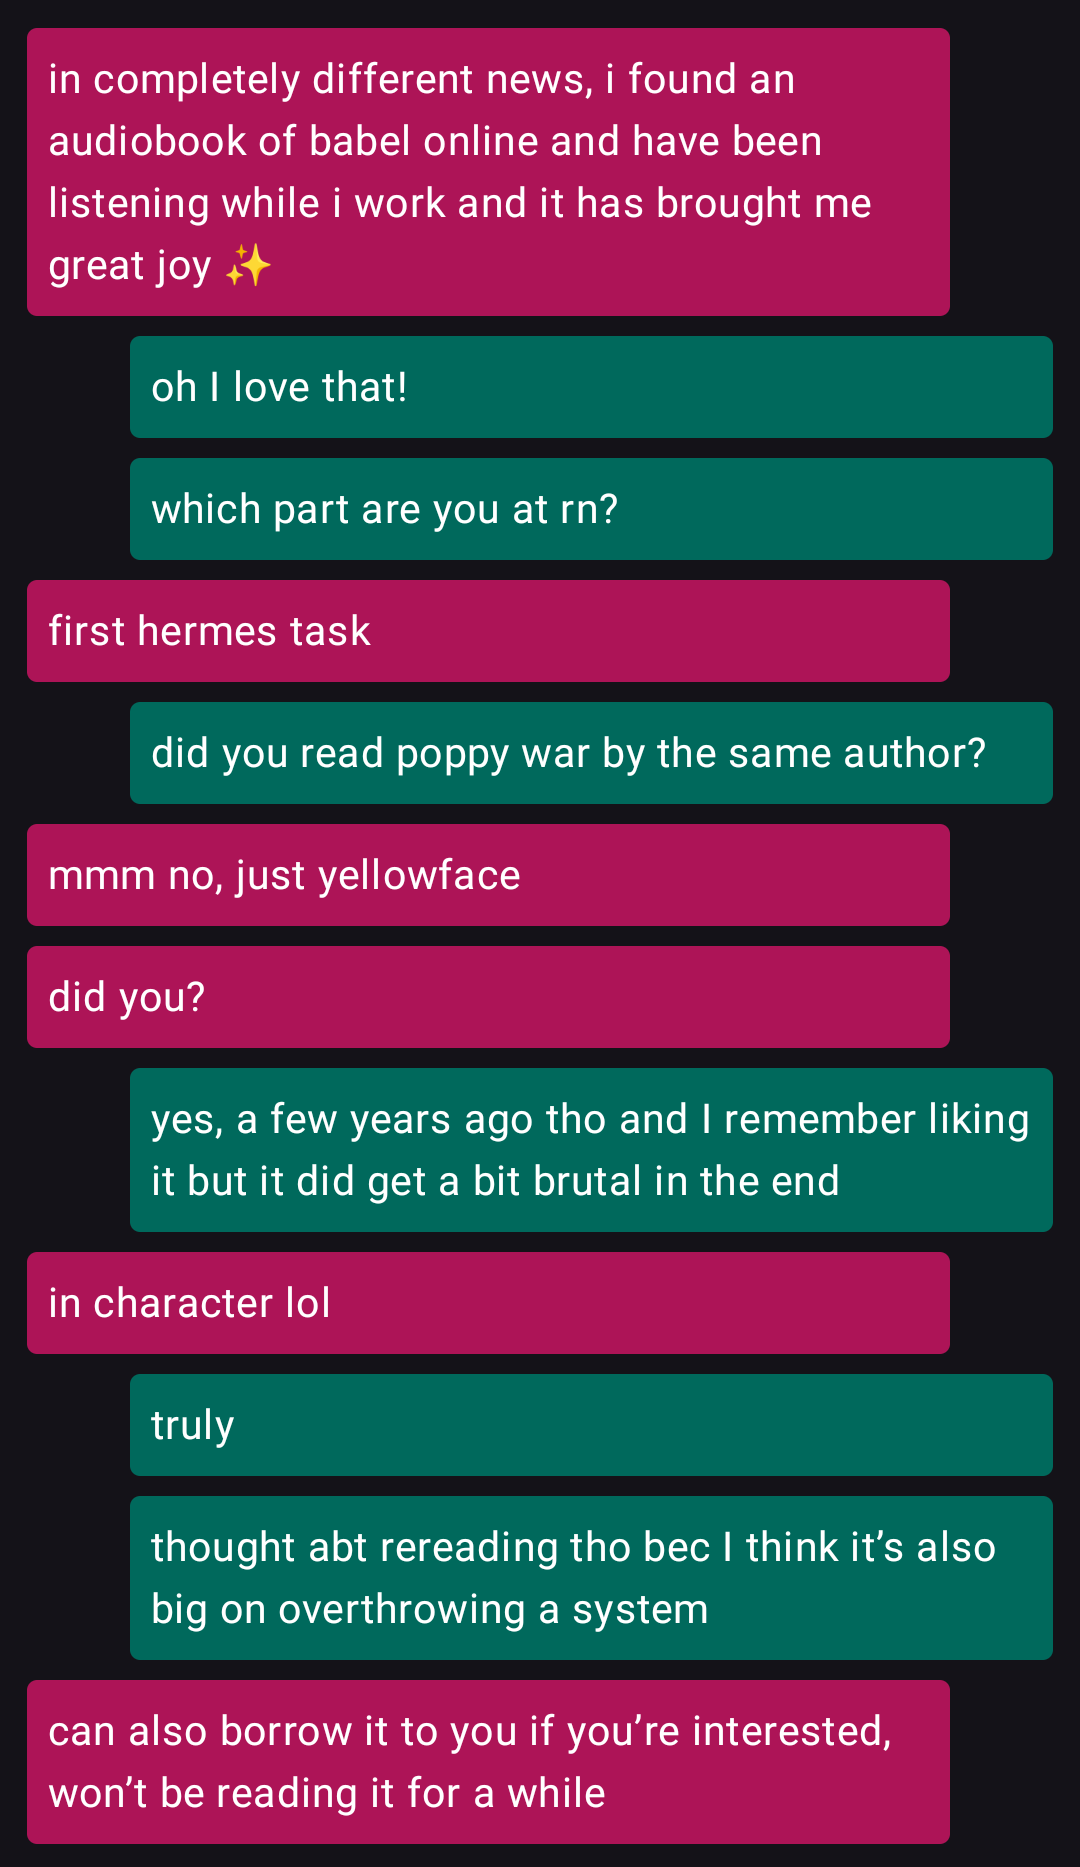
\includegraphics[width=\linewidth]{survey_real_2.png}
		\caption{Real chat conversation.}
		\label{fig:surveyReal2}
	\end{subfigure}

	\caption[Survey: Chats]{The chat conversations we used in our survey, both real and cover texts.}
	\label{fig:survey}
\end{figure}

\begin{table}
	\centering
	\begin{tabular}{@{} ll @{}} % @{} removes white spaces
		\toprule
		\tableheadline{Chat} & \tableheadline{System prompt} \\
		\midrule
        Arithmetic & \\
		\midrule
        \cref{fig:surveyArithmetic1} & \parbox{10cm}{"Let's do a role play. You and I are friends, texting with each other. We are talking about going to a concert. Be brief and casual, but friendly and engaging. Use emojis and phrases typical for chat messages."} \\
		\addlinespace[0.25cm] % Add some space between rows
		\cref{fig:surveyArithmetic2} & \parbox{10cm}{"Let's do a role play. You and I are a couple, texting with each other. We are planning a date night together. Be brief and casual, but friendly and engaging. Use emojis and phrases typical for chat messages."} \\
        \midrule
        Huffman & \\
        \midrule
        \cref{fig:surveyHuffman1} & \parbox{10cm}{"Let's do a role play. You and I are construction workers, texting with each other. We are talking about the next day at work. Be brief and casual, but friendly and engaging. Use some emojis and phrases typical for chat messages, but not too many."} \\
		\addlinespace[0.25cm] % Add some space between rows
		\cref{fig:surveyHuffman2} & \parbox{10cm}{"Let's do a role play. You and I are a couple, texting with each other. We are planning the birthday party for our child. Be brief and casual, but friendly and engaging. Use emojis and phrases typical for chat messages."} \\
		\bottomrule
	\end{tabular}
	% Use alternative short title for table of contents
	\caption[Survey: System prompts]{The system prompts we used to generate the cover texts for our survey.}
	\label{tab:systemPrompts}
\end{table}
